%
%\section{Présentation}
%\ifprof
%\else
%Après des années de recherche et de développement puis un voyage de 485 millions de kilomètres, la sonde InSight (Interior Exploration using Seismic Investigations, Geodesy and Heat Transport) s'est posée sur Mars le 26 novembre 2018. Elle est le premier observatoire géophysique martien, dont l'objectif est d'étudier la structure interne de Mars et de comprendre la formation et l'évolution des planètes rocheuses du Système solaire. En mesurant la façon dont les ondes sismiques, provoquées par des séismes martiens ou des impacts de météorites, se propagent à l'intérieur de Mars, les géophysiciens vont pouvoir répondre avec précision à cet objectif.
%
%\begin{figure}[!h]
%\centering
%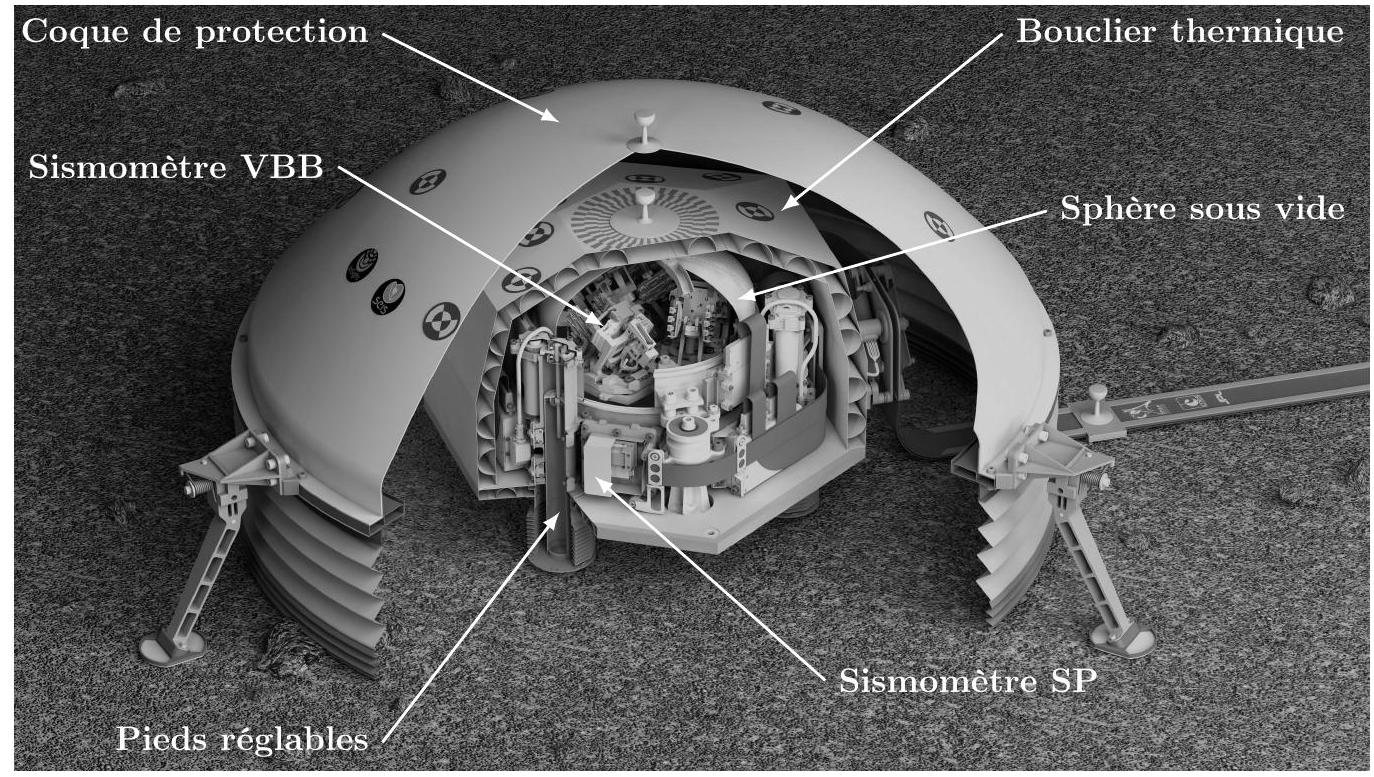
\includegraphics[width=.6\textwidth]{2024_04_26_3285cfc264024262add0g-02}
%\caption{\label{ccmp2023_fig_01}Écorché de SEIS et ses différents niveaux de protection}
%%FigURE 1 - Écorché de SEIS et ses différents niveaux de protection}
%\end{figure}

\section{Performances de l'asservissement}
\ifprof
\else
SEIS comporte deux sismomètres indépendants, le VBB (Very Broad Band) et le SP (Short Periods), montés sur une structure commune pouvant être réglée à l'horizontale grâce à des pieds de longueur variable.

\begin{itemize}
  \item Le sismomètre VBB comporte trois systèmes identiques, composés chacun d'un pendule et d'un bâti, inclinés différemment par rapport au sol. Ils sont fixés dans une sphère en titane sous vide, et sensibles à une large bande de fréquence d'ondes sismiques, entre \SI{0,01}{Hz} et $0,5 \si{Hz}$.
  \item Le sismomètre SP est adapté aux ondes sismiques de plus hautes fréquences, entre 0,1 et $50 \si{Hz}$.
\end{itemize}

\begin{figure}[!h]
\centering
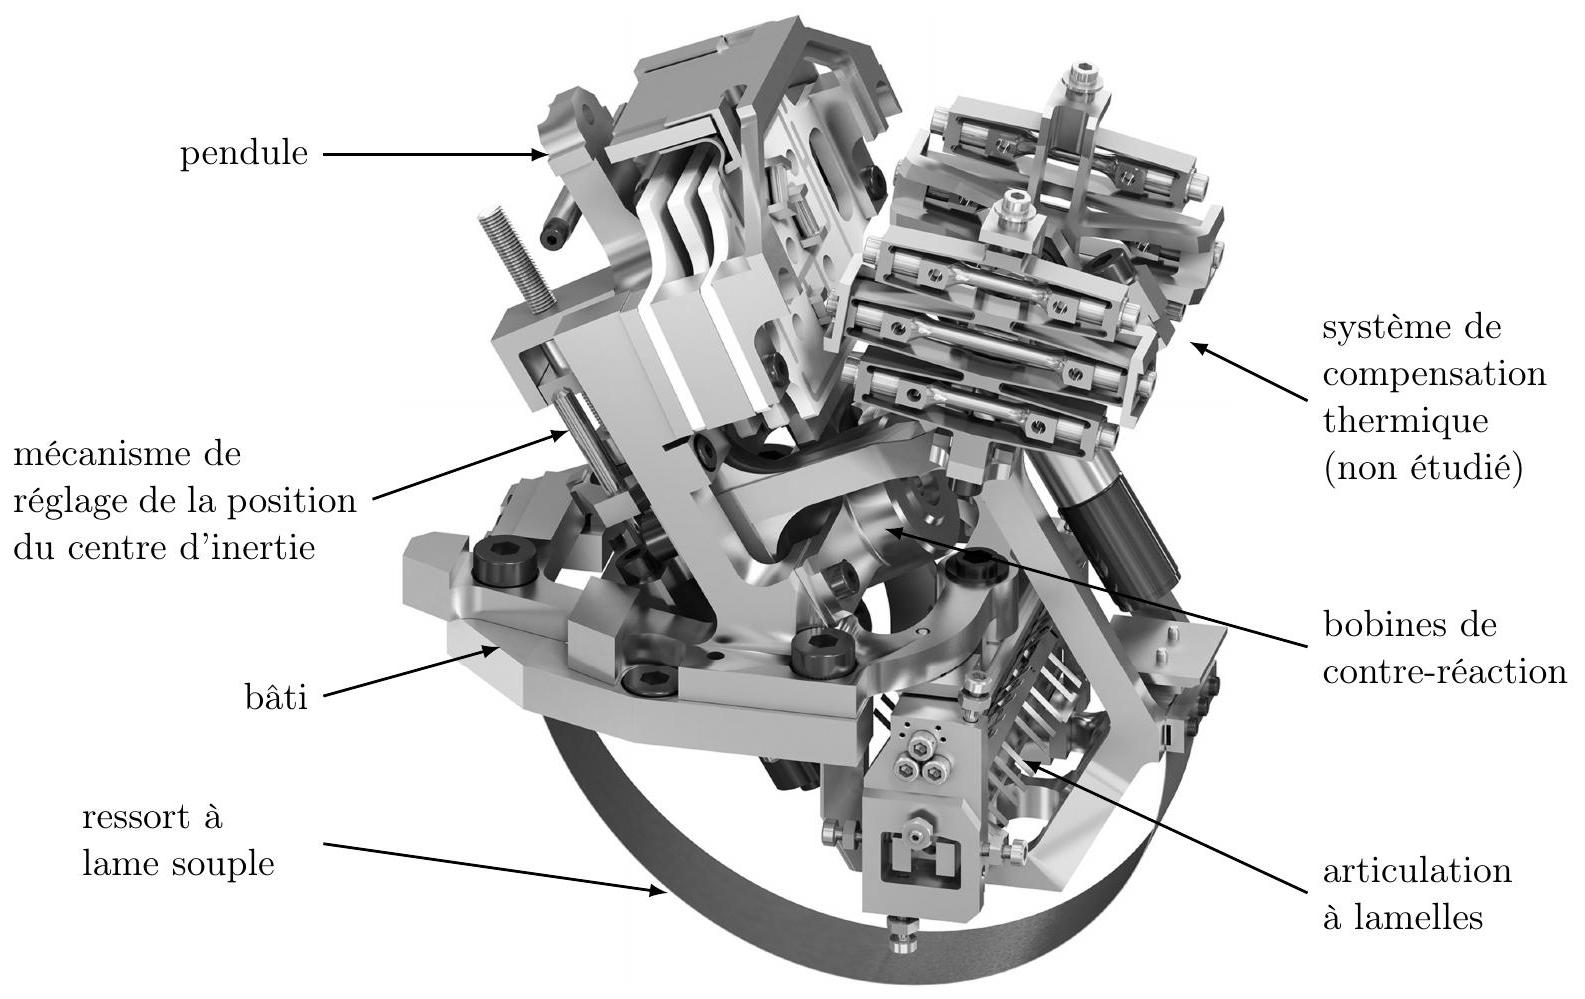
\includegraphics[width=.7\textwidth]{2024_04_26_3285cfc264024262add0g-03}
\caption{\label{ccmp2023_fig_02} Vue 3D d'un des trois systèmes du VBB}
% Figure 2 - Vue 3D d'un des trois systèmes du VBB
\end{figure}


Une vue détaillée d'un des systèmes du VBB est fournie en figure \ref{ccmp2023_fig_02} et le détail des différents éléments qui le constituent est fourni en Annexe 1.

L’équilibre de l’ensemble mobile sur Terre peut s'exprimer par l'équation suivante : 
$ aM_2 g_M \sin\indice{\alpha}{eq} +C_0 - k( \indice{\alpha}{eq} -\alpha_0)=0 $(eq. 1).
\fi



\ifprof
\else
À chaque mouvement du sol, un capteur mesure la position angulaire du pendule (2) par rapport au bâti (1). Des bobines de contre-réaction situées sur le pendule (voir figure \ref{ccmp2023_fig_02} et l'Annexe 1) génèrent un moment de rappel sur son axe de rotation, qui le ramène à sa position d'équilibre.

\begin{itemize}
  \item La bobine HF (pour Haute Fréquence) pilote l'asservissement entre 0,05 Hz et 0,5 Hz. Son rôle principal est d'amortir les secousses trop brusques et d'éliminer la résonance du pendule.
  \item La bobine BF (pour Basse Fréquence) a été conçue pour intervenir sur les fréquences inférieures à $0,05 \si{Hz}$. Elle permet de filtrer la variation journalière de température et les dérives saisonnières plus lentes.
\end{itemize}

L'asservissement mis en place est donc une régulation devant permettre d'annuler en régime permanent les effets des secousses sismiques sur le pendule, tout en étant sensible aux signaux dans une large bande de fréquences d'ondes sismiques, entre $0,01 \si{Hz}$ et $0,5 \si{Hz}$.

Les exigences auxquelles doit répondre cet asservissement sont fournies dans la table \ref{ccmp2023_tab_03}.

\begin{table}[!h]
\centering
\begin{tabular}{cp{5cm}p{5cm}p{5cm}}
\hline
$\mathbf{3}$ & \multicolumn{3}{l}{Acquérir les vibrations du sol martien}  \\
\hline
$\mathbf{3.1}$ &\multirow{2}{4cm}{Éliminer la résonance du système tout en maintenant une rapidité maximale}&
Résonance du système avec l'action de la bobine HF seule &  aucune \\
\cline { 3 - 4 }
& & Rapidité du système avec l'action de la bobine HF seule & bande passante à $-3 \si{dB}$ maximale \\
\hline
$\mathbf{3 . 2}$ & 
Ramener le déplacement du pendule à zéro 
& Précision de l'asservissement en tension & écart statique nul en réponse à un échelon d'accélération du sol \\
\hline
$\mathbf{3 . 3}$ & Filtrer le signal & Amplification des mouvements du sol par l'asservissement en tension & 
$\geq 110 \si{dB}$ limitée à la bande $[0,06 ; 3]$ \si{rad} $\mathrm{s}^{-1}$ \\
\hline
$\mathbf{3 . 4}$ & Éviter des problèmes de saturation & Amplification des mouvements du sol par l'asservissement en tension 
&$<120 \si{dB}$ pour tous les signaux mesurés \\
\hline
\end{tabular}
\caption{\label{ccmp2023_tab_03}  Liste (non exhaustive) des exigences de l'asservissement}
%TABLE 3 - Liste (non exhaustive) des exigences de l'asservissement
\end{table}



\begin{obj}
Régler la correction des bobines $\mathrm{HF}$ et $\mathrm{BF}$.
\end{obj}

Le réglage de l'asservissement s'effectue par une étude numérique, dans les conditions de la gravité martienne. On considère donc le pendule (2) sans son contrepoids (3). On note $J$ le moment d'inertie du pendule (2) sur l'axe ( $\left.O_{1}, \overrightarrow{z_{1}}\right)$. Pour simplifier l'étude, on néglige les frottements dans l'articulation à lamelles, et on note $K=k-d M g_{M} \cos \alpha_{0}$ la raideur équivalente du pendule.

La grandeur utile aux scientifiques qui analysent les données mesurées par le sismomètre est la tension électrique en sortie du capteur, image de la position angulaire du pendule autour de sa position d'équilibre.

Le schéma-blocs de l'asservissement en tension d'un système est fourni en Annexe 5 , ainsi que la description des grandeurs physiques intervenant dans l'asservissement et les données numériques utiles à cette partie.

On s'intéresse dans un premier temps à l'asservissement avec l'action de la bobine HF seule. Le schéma-blocs correspondant est fourni à la figure \ref{ccmp2023_fig_11}.

\begin{figure}[!h]
\centering
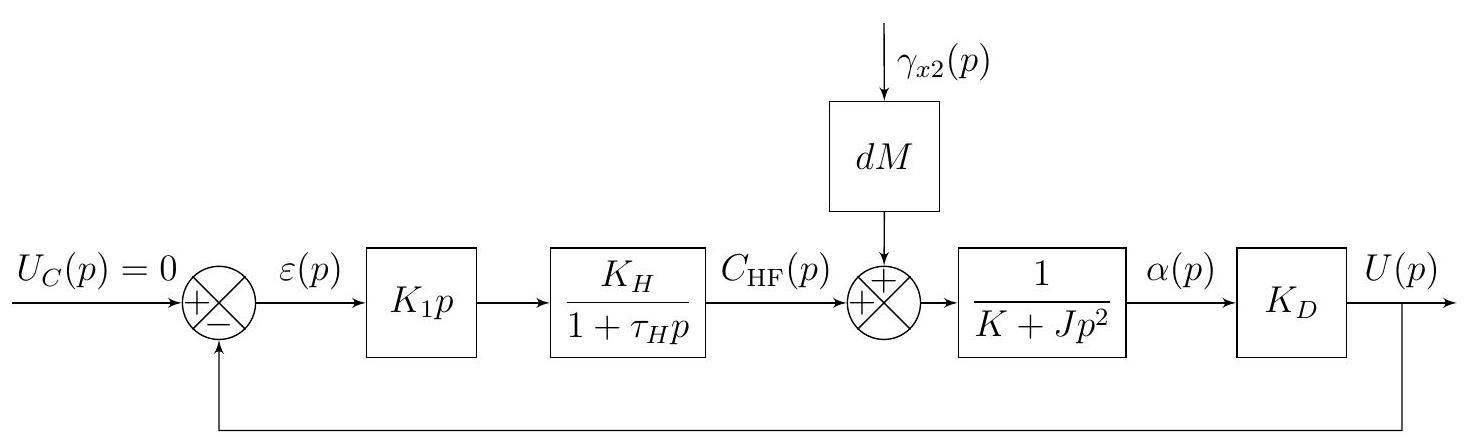
\includegraphics[width=\textwidth]{2024_04_26_3285cfc264024262add0g-13(1)}
\caption{\label{ccmp2023_fig_11} Schéma-blocs de l'asservissement avec l'action de la bobine HF seule}
\end{figure}
\fi

%FIGURE 11 - Schéma-blocs de l'asservissement avec l'action de la bobine HF seule

\question{\label{ccmp2023_q_23}. Déterminer la fonction de transfert $H_{\gamma}(p)=\frac{U(p)}{\gamma_{x 2}(p)}$, avec $U_{C}(p)=0$, en l'exprimant sous la forme:
$
H_{\gamma}(p)=K_{\mathrm{HF}} \cdot \frac{1+a_{1} p}{1+b_{1} p+b_{2} p^{2}+b_{3} p^{3}}
$
où l'on précisera les expressions de $K_{\mathrm{HF}}, a_{1}, b_{1}, b_{2}$ et $b_{3}$.}
\ifprof
\begin{corrige}
\textbf{[UPSTI]} --
D’après la formule de Black, on a :
$H_{\gamma} (p)=dM \dfrac{\dfrac{K_D}{K+Jp^2}}{1+\dfrac{K_D K_H K_1 p}{(K+Jp^2)(1+\tau_H p)}}$

$H_{\gamma} (p)=dM \dfrac{\dfrac{K_D}{K+Jp^2}}{\dfrac{(K+Jp^2)(1+\tau_H p)+K_D K_H K_1 p}{(K+Jp^2)(1+\tau_H p)}}$

$H_{\gamma} (p)=dM \dfrac{K_D}{K+Jp^2}  \dfrac{(K+Jp^2)(1+\tau_H p)}{(K+Jp^2)(1+\tau_H p)+K_D K_H K_1 p}$

$H_{\gamma} (p)=dMK_D  \dfrac{1+\tau_H p}{(K+Jp^2)(1+\tau_H p)+K_D K_H K_1 p}$

$H_{\gamma} (p)=dMK_D  \dfrac{1+\tau_H p}{J\tau_H p^3+Jp^2+(K\tau_H+K_D K_H K_1)p+K}$

$H_{\gamma} (p)=\dfrac{dMK_D}{K}  \dfrac{1+\tau_H p}{1+(K\tau_H+K_D K_H K_1)/K p+J/K p^2+(J\tau_H)/K p^3  }$

Par identification, on a :
$K_HF=\dfrac{dMK_D}{K}$, 
$a_1=\tau_H$, 
$b_1=\dfrac{K\tau_H+K_D K_H K_1}{K}$, 
$b_2=\dfrac{J}{K}$, 
$b_3=\dfrac{J\tau_H}{K}$.

\end{corrige}
\else
\fi

\ifprof
\else
On donne les pôles $p_{i}$ de $H_{\gamma}(p)$ en table \ref{ccmp2023_tab_04} et le diagramme de Bode en gain de $H_{\gamma}(p)$ en figure \ref{ccmp2023_fig_12} pour différentes valeurs de $K_{1}$.


\begin{table}[!h]
\centering
\begin{tabular}{|c|c|c|c|}
\hline
$K_{1}$ & $p_{1}$ & $p_{2}$ & $p_{3}$ \\
\hline\hline
0,05 & $-1000$ & $$-0,38-2,33$ \mathrm{j}$ & $-0,38+2,33 \mathrm{j}$ \\
\hline
0,5 & $-1000$ & $-0,64$ & $-9,32$ \\
\hline
5 & $-1000$ & $-0,069$ & $-95,7$ \\
\hline
\end{tabular}
\caption{\label{ccmp2023_tab_04} Pôles de la fonction de transfert $H_{\gamma}(p)$ }
\end{table}

%TABLE 4 - Pôles de la fonction de transfert $H_{\gamma}(p)$

\begin{figure}[!h]
\centering
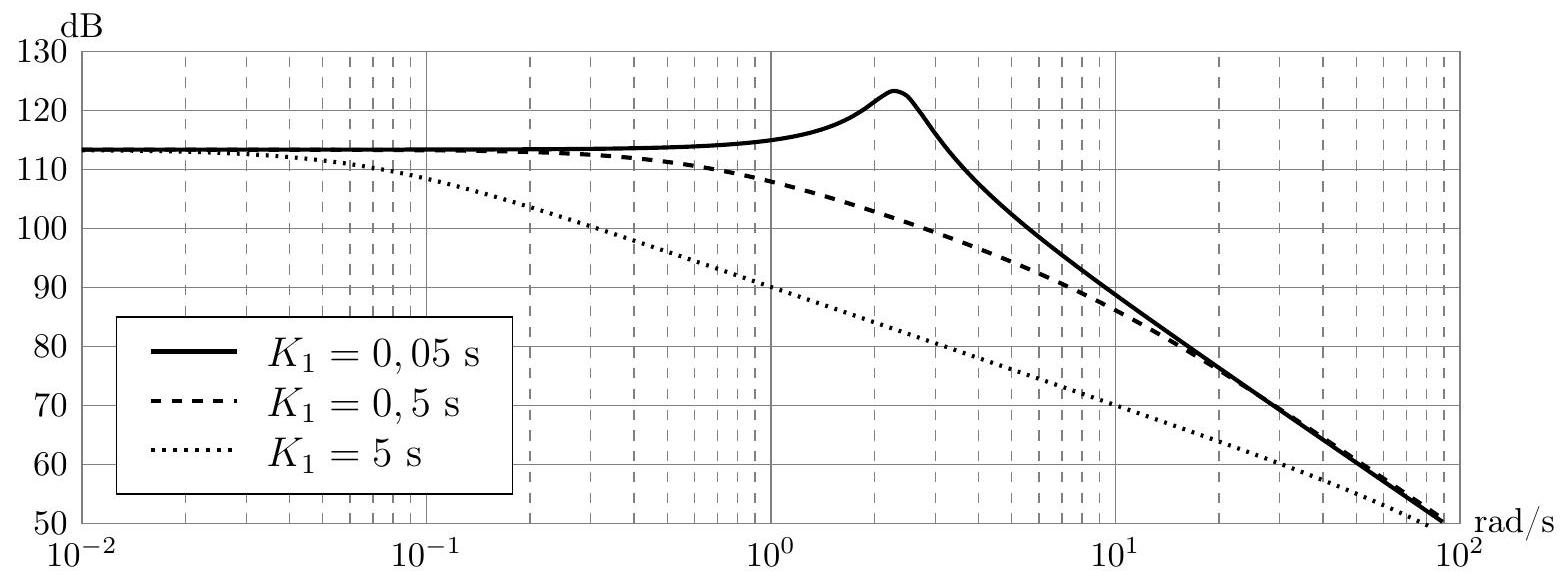
\includegraphics[width=\textwidth]{2024_04_26_3285cfc264024262add0g-13}
\caption{\label{ccmp2023_fig_12} Diagramme de Bode en gain de la fonction de transfert $H_{\gamma}(p)$}
%Figure 12 - Diagramme de Bode en gain de la fonction de transfert $H_{\gamma}(p)$
\end{figure}

Le réglage du correcteur HF doit permettre de répondre à l'exigence 3.1.
\fi

%Q24. 
\question{\label{ccmp2023_q_24}Justifier que $H_{\gamma}(p)$ correspond à un système stable quelle que soit la valeur retenue pour $K_{1}$ dans la gamme $[0,05 ; 5]$ s. Choisir, en justifiant, la valeur de $K_{1}$ parmi les valeurs proposées, la plus adaptée au réglage de l'asservissement avec l'action de la bobine HF seule.}
\ifprof
\begin{corrige}
\textbf{[UPSTI]} --
Tous les pôles ont des parties réelles strictement négatives. On en déduit que le système est stable au sens entrée bornée-sortie bornée.

L’exigence 3.4 n’est pas respectée pour une valeur de K1 de 0,05 (gain supérieur à 120 dB). On cherche une bande passante la plus grande possible pour respecter l’exigence 3.1. On choisit donc une valeur de K1 de 0,5.
\end{corrige}
\else
\fi

%Q25. 
\question{\label{ccmp2023_q_25}En s'appuyant sur les données numériques de la table \ref{ccmp2023_tab_04} et de l'Annexe 5, justifier que, pour la valeur retenue de $K_{1}$, la fonction de transfert peut s'écrire sous la forme :
$$
H_{\gamma}(p)=\frac{d M K_{D}}{K} \cdot \frac{1}{\left(1+\tau_{2} p\right)\left(1+\tau_{3} p\right)}, \text { avec } \tau_{2} \gg \tau_{3}
$$
Préciser les valeurs des constantes de temps $\tau_{2}$ et $\tau_{3}$.}

\ifprof
\begin{corrige}%
\textbf{[UPSTI]} -- 
$\tau_1=-\dfrac{1}{p_1} =\dfrac{1}{1000}\si{s^{-1}}$,  $\tau_2=-1/p_2 =1/0,64 \si{s^{-1}}$,  $\tau3=-1/p_3 =1/9,32\si{s^{-1}}$. 

On constate que $\tau_2 >> \tau_1$ et $\tau_3>> \tau_1$. Le pôle $p_1$ pourrait être négligé (constante de temps très faible par rapport aux autres. Mais ici il se simplifie avec le zéro de la fonction de transfert ($\tau_1=\tau_H$) et 
$H_{\gamma} (p)= \dfrac{dMK_D}{K} \dfrac{ 1}{(1+\tau2 p)(1+\tau3 p)}$

\end{corrige}
\else
\fi


Pour la suite des questions, on conservera cette forme simplifiée de $H_{\gamma}(p)$.

%Q26. 
\question{\label{ccmp2023_q_26}Justifier que l'asservissement avec l'action de la bobine HF seule ne permet pas de satisfaire les exigences 3.2 et 3.3.}
\ifprof
\begin{corrige}%
\textbf{[UPSTI]} -- 
L’exigence 3.2 impose un écart statique nul en réponse à un échelon d’accélération du sol. Cette exigence n’est pas satisfaite. Pour le justifier :
	Soit remarquer qu’il n’y a pas d’intégration en amont de la perturbation, l’écart statique vis-à-vis de cette perturbation est donc non nul.
	Soit calculer la limite de l’écart lorsque t tend vers l’infini avec $u_c (t)=0$ et $\gamma_{x2} (t)= \gamma_0 u(t)$ 
	$$ \lim_{t\to\infty}  \varepsilon(t) 
	= \lim_{p\to 0}  pU(p) 
	= \lim_{p\to 0}-H_{\gamma} (p) \gamma_0 =-\dfrac{dMK_D}{K} \gamma_0 \neq 0.$$

Le gain n’est pas supérieur à \SI{110}{dB} sur toute la gamme de fréquence. On en déduit que l’exigence 3.3 n’est pas respectée non plus.

\end{corrige}
\else
\fi

\ifprof
\else
En tenant compte des résultats précédents, le schéma-blocs de l'Annexe 5 peut se mettre sous la forme de celui de la Figure \ref{ccmp2023_fig_13}.

\begin{figure}[!h]
\centering
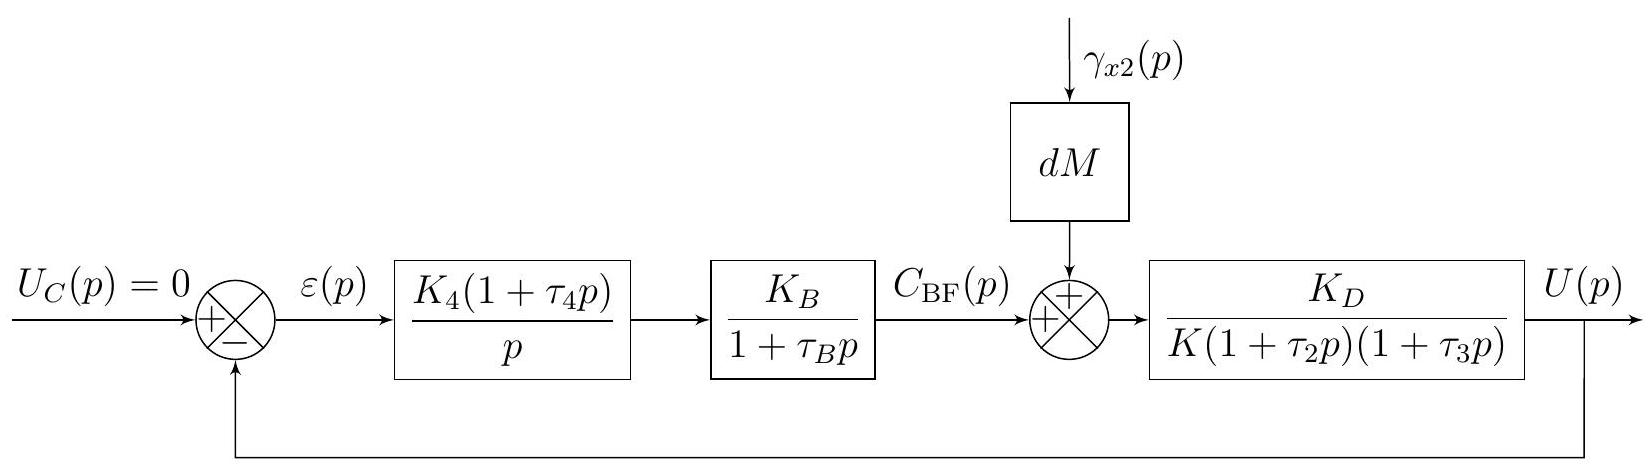
\includegraphics[width=\textwidth]{2024_04_26_3285cfc264024262add0g-14}
\caption{\label{ccmp2023_fig_13}  Schéma-blocs de l'asservissement d'un système}
%FigURe 13 - Schéma-blocs de l'asservissement d'un système
\end{figure}



Le correcteur BF est un correcteur proportionnel intégral. Pour optimiser la rapidité, $\tau_{4}$ doit permettre de compenser le pôle dominant de la boucle ouverte. $K_{4}$ est réglé de façon à répondre aux exigences 3.3 et 3.4.
\fi

%Q27. 
\question{\label{ccmp2023_q_27}Préciser l'intérêt de la chaîne d'action BF vis-à-vis de l'exigence 3.2.}
\ifprof
\begin{corrige}%
\textbf{[UPSTI]} -- L’action BF permet d’augmenter la classe de la FTBO. Il y a une intégration en amont de la perturbation, l’écart statique vis-à-vis de cette perturbation est donc nul. L’exigence 3.2. est satisfaite.
\end{corrige}
\else
\fi

%Q28. 
\question{\label{ccmp2023_q_28}Donner l'expression de la fonction de transfert en boucle ouverte de l'asservissement, $H_{B O}(p)=\frac{U(p)}{\varepsilon(p)}$. Donner, en justifiant, la valeur retenue pour $\tau_{4}$.}
\ifprof
\begin{corrige}%
\textbf{[UPSTI]} -- 
$\indice{H}{BO} (p)=\dfrac{K_D K_4 K_B (1+\tau_4 p)}{Kp(1+\tau_B p)(1+\tau_2 p)(1+\tau_3 p)}$
On cherche à éliminer le pôle dominant. On a donc : $\tau_4=\tau_2$ et  
$\indice{H}{BO} (p)=\dfrac{K_D K_4 K_B}{Kp(1+\tau_B p)(1+\tau_3 p)}$

\end{corrige}
\else
\fi

\ifprof
\else
On donne, pour la valeur de $\tau_{4}$ retenue et différentes valeurs de $K_{4}$, le diagramme de Bode de l'asservissement en tension, $\frac{U(p)}{\gamma_{x 2}(p)}$, sur la Figure ci desssous. %C du document réponse (question \ref{ccmp2023_q_29}).
\fi

\ifprof
\else
\begin{figure}[!h]
\centering
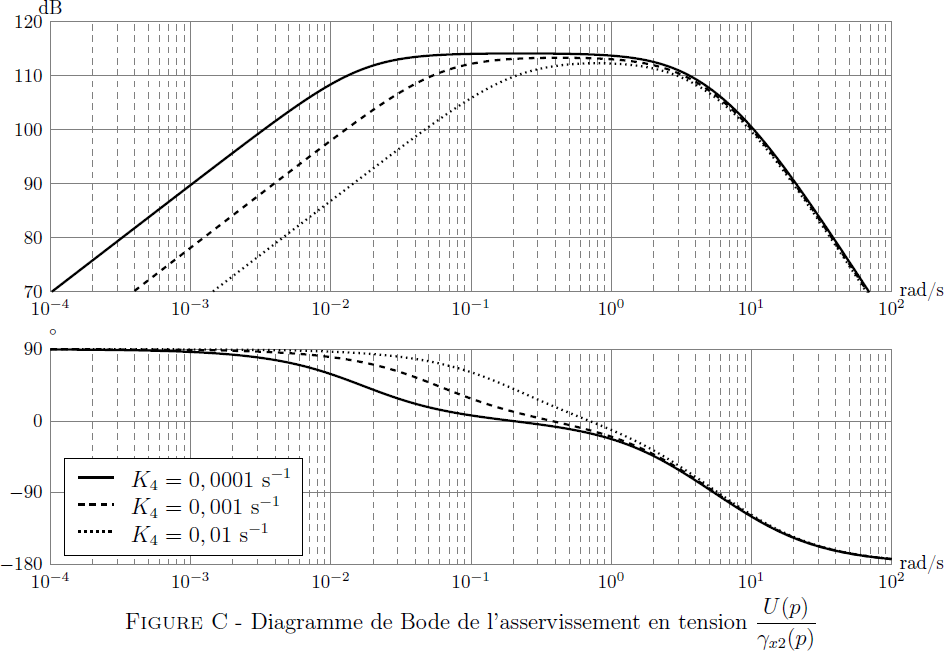
\includegraphics[width=\textwidth]{DR_29_C}
%\caption{\label{ccmp2023_fig_13}  Schéma-blocs de l'asservissement d'un système}
%FigURe 13 - Schéma-blocs de l'asservissement d'un système
\end{figure}
\fi

%Q29. 
\question{\label{ccmp2023_q_29}Choisir, en justifiant, la valeur de $K_{4}$ qui permet de vérifier au mieux les exigences 3.3 et 3.4.}
% Les tracés nécessaires apparaitront sur le document réponses.}
\ifprof
\begin{corrige}%
\textbf{[UPSTI]} --
Pour $K = \SI{0,0001}{s^{-1}}$, on amplifie (Gain $\geq \SI{110}{dB}$) sur une bande $\left[0,01 ; 3\right] \si{rad/s}$.
Pour $K = \SI{0,01}{s^{-1}}$, on amplifie sur une bande $\left[0,2 ; 3\right] \si{rad/s}$.
On choisit donc une valeur de $K$ de $\SI{0,001}{s^{-1}}$ (on amplifie sur une bande $\left[0,06 ; 3\right] \si{rad/s}$).

\end{corrige}
\else
\fi

%Q30. 
\question{\label{ccmp2023_q_30}Donner le nom du type de filtre réalisé par le pendule asservi et préciser l'intérêt de cette solution pour la mesure des séismes par le sismomètre VBB.}
\ifprof
\begin{corrige}%
\textbf{[UPSTI]} -- 
Il s’agit d’un filtre passe bande. Il permet de sélectionner les fréquences souhaitées en amplifiant uniquement ces dernières.
\end{corrige}
\else
\fi


